\section{Physarum Polycephalum}
\label{section:background_physarum}

The organism being a subject for this work is \textit{Physarum Polycephalum} also called the many-headed slime mould. It is a member of the \textit{Physaridae} family of slime moulds, in order of \textit{Physarales}, class \textit{Myxogastria}, phylum \textit{Myxomycete}, supergroup \textit{Amoebozoa} in \textit{Protista} kingdom. While current position in taxology is well defined, presented characteristics will justify why scientists used to have problems with classification of the Physarum \cite{stephenson1994myxomycetes}.

In order to make the thesis readable, terms \textit{Physarum Polycephalum}, \textit{Physarum} or \textit{the slime mould} will be used interchangeably as the subject is unambiguously defined. As none of the authors have a background in biology, concepts are presented from a computer scientist's perspective in minimal, yet exhaustive, form.


\subsection{Biological characteristics}

\textit{Physarum Polycephalum} is a very peculiar organism. Even being a \textit{Protista} it can be observed with a naked eye --- it is a one amongst biggest living unicellular ogranisms \cite{TODO}. 

In its natural habitat, under cool, dark and humid conditions the slime mould exists in form of a yellow structurized blob (as seen in figure \ref{figure:bp_habitat}). Its occurrence is fairly common around the globe, however species \textit{Physarum Polycephalum} does not occur naturally in Poland \cite{narkiewicz2013grzyby}. It feeds on bacteria, fungi and other sources of basic nutrients.

In labaratory conditions, \textit{Physarum} is stored on Petri dishes filled with non-nutritious agar. The agar base provides humid environment required for supporting plasmodial stage of the slime mould. A sterille oats or even soft porridge is used as controlled source of nutrients. Complete description of storage and observing environment, among other informations, is provided in Appendix \ref{chapter:protocol}.

% TODO find another image
\begin{figure}
  \centering
  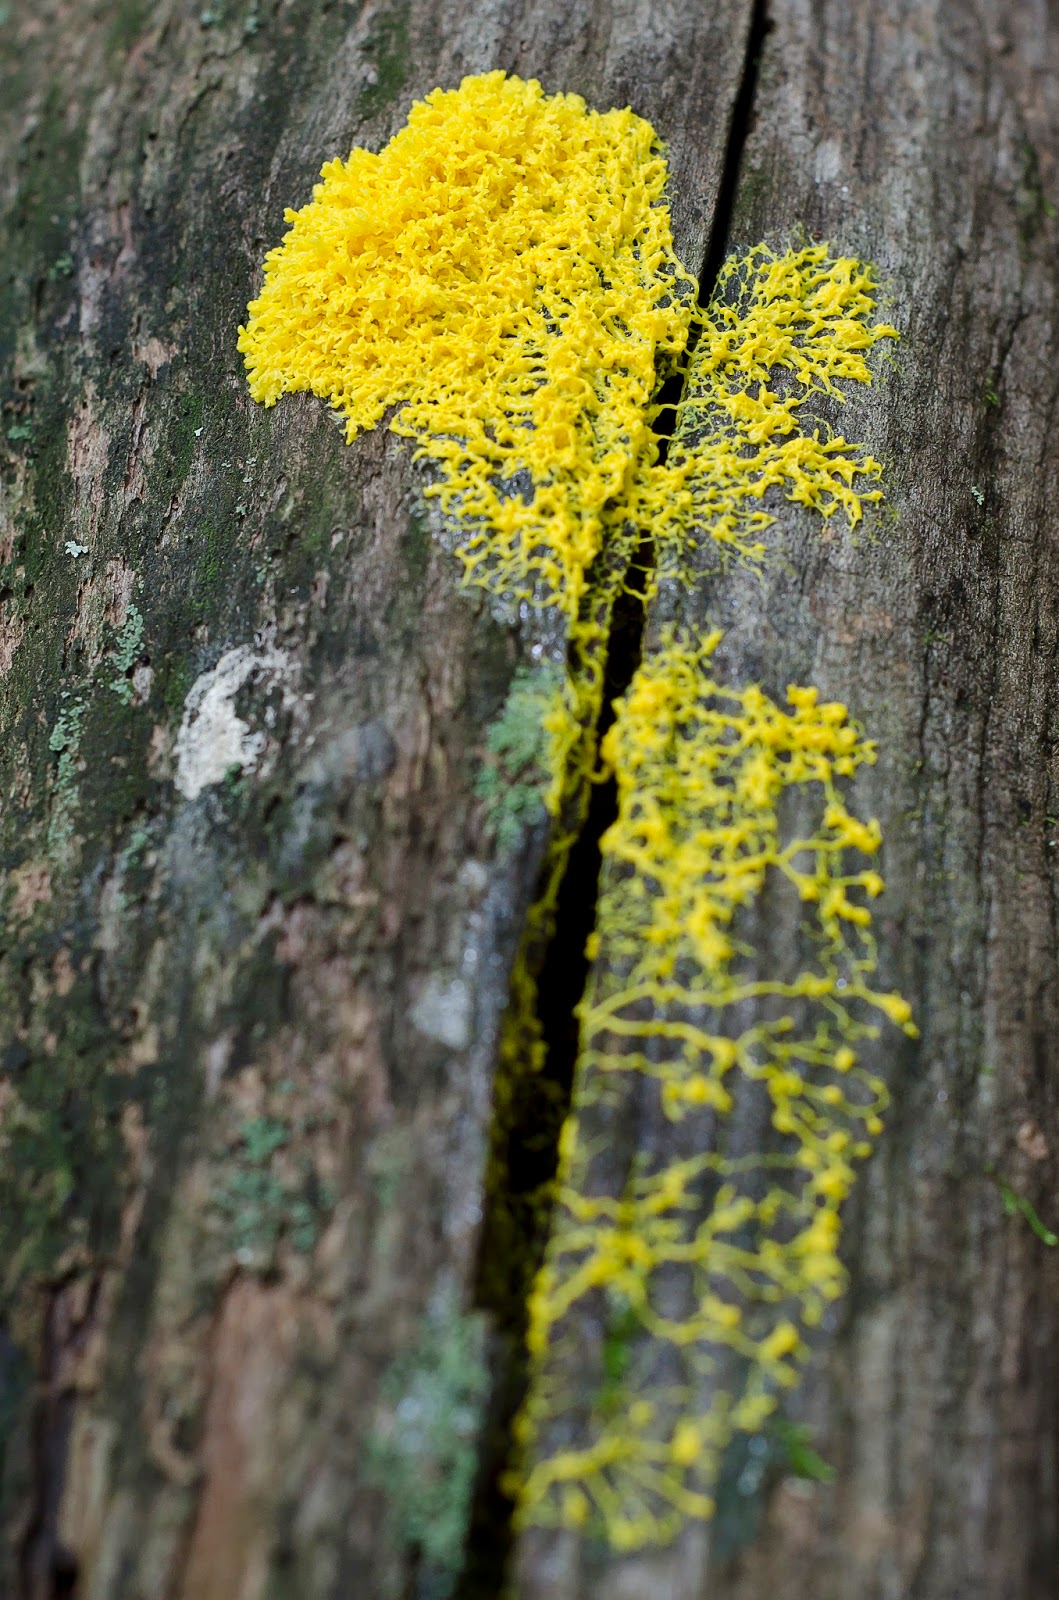
\includegraphics[width=0.44\textwidth]{background/physarum/habitat.jpg}
  \caption{\textit{Physarum Polycephalum} in its habitat \cite{TODO}}
  \label{figure:bp_habitat}
\end{figure}

\begin{figure}
  \centering
  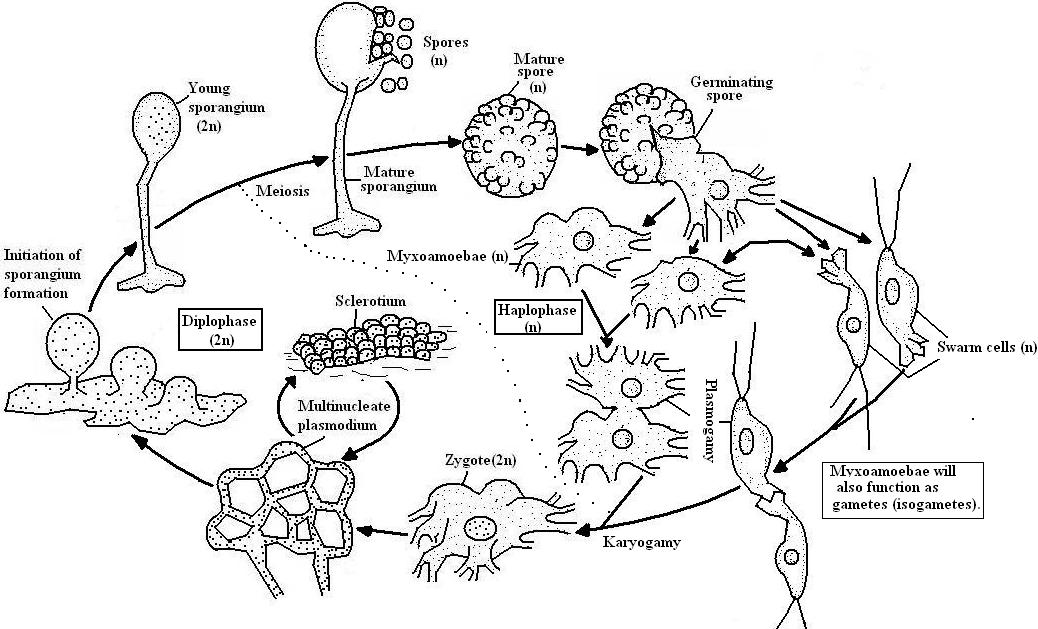
\includegraphics[width=0.94\textwidth]{background/physarum/lifecycle.png}
  \caption{Lifecycle of \textit{Physarum Polycephalum} \cite{TODO}}
  \label{figure:bp_lifecycle}
\end{figure}

As representant of \textit{Myxomycete}, a life cycle of the slime mould is very complex (as seen in figure \ref{figure:bp_lifecycle}). For purposes of unconventional computing applications, \textit{Physarum} is preferred in its plasmodial stage. However, during research transformations into other states are inevitable and must be dealt with.


\subsection{Observations}

lorem


\subsection{Emerging computational possibilities}

lorem


\subsection{Interaction}

lorem

